\documentclass[../main.tex]{subfiles}

\begin{document}
	\paragraph{}L'application Android a été développée sous l'IDE Android Studio 3, avec l'API Android 16, supportant ainsi près de 99\% des appareils Android en circulation. Le code de l'application a été entièrement géré avec Git et est d'ailleurs disponible à l'adresse suivante : \url{https://github.com/tndnc/pandroid/tree/master/equity}. 
	
	L'application devait répondre aux spécifications suivantes: permettre aux utilisateurs de sélectionner des niveaux, de les résoudre et d'en noter la difficulté. Pour les administrateurs il était également important de pouvoir facilement mettre à jour la liste des niveaux ainsi que de pouvoir récupérer les notes et meta-données issues de l'utilisation de l'application par les utilisateurs. Ces données devaient pouvoir être exportées vers une base données Google Sheets.
	% Google sheets API v4 à ajouter dans partie sur google sheet.
	
	\subsection{Composants Android}
	Une application Android s'organise en plusieurs composants, nous allons en présenter certains dans la~\Cref{sec-struct} pour pouvoir décrire l'application et ses fonctionnalités aisément. Nous allons notamment nous concentrer sur le concept d'activité, nécessaire pour pouvoir présenter l'interface.
	
	Une activité Android correspond à une fenêtre d'application et chaque application est donc composée d'au moins une activité. La navigation à l'intérieur d'une application se fait en changeant d'activité. Leur apparence visuelle est principalement définie par leur \textit{layout} qui structure l'agencement des vues (images, boutons, etc) et peut lier certains événements, initiés par l'utilisateur (comme par exemple un \textquote{clic} de bouton), à des actions prédéfinies (par exemple, lancer un niveau). Le layout, chargé par une activité à sa création, est décrit dans un fichier XML.
	
	\subsection{Structure de l'application}
	\label{sec-struct}
Notre application est composée de six activités que nous allons présenter ici. Des impressions d'écrans sont visibles en~\Cref{fig-screen1}.
\hfill \break
\begin{itemize}
 \item \texttt{MainMenuActivity} : l'activité principale de l'application, lorsque celle-ci est ouverte, l'utilisateur arrive sur l'écran qui correspond au menu principal, il a ensuite la possibilité de sélectionner un des quatres boutons du layout pour effectuer les actions suivantes : ouvrir le menu de sélection des niveaux, lancer le tutoriel, modifier son profil utilisateur ou ouvrir la page \textquote{à propos}.
 \item \texttt{LevelSelectActivity} : l'activité de sélection des niveaux dans laquelle la liste des niveaux est affichée, catégorisée par le nombre d'agents de chacun des niveaux. L'utilisateur a la possibilité de lancer chacun des niveaux présentés.
 \item \texttt{UserProfileActivity} : Cette activité remplace la \texttt{MainMenuActivity} lors du premier lancement de l'application. Elle comporte deux zones d'entrées de texte qui permettent à l'utilisateur de rentrer sa formation et son âge, données utiles lors de l'analyse des niveaux. On note que l'utilisateur a la possibilité de revenir sur cette activité depuis le menu principal ou de ne pas remplir les champs de texte s'il ne désire pas partager ces informations. 
 \item\texttt{AboutActivity} : un bref résumé de l'objectif de notre projet et des raisons pour laquelle l'application a été développé est visible sur cette page.
 \item\texttt{TutorialActivity} : le tutoriel du jeu, on y trouve une description de l'interface de jeu, la définition de ce qu'est un agent jaloux, les modalités de victoire d'une partie ainsi que des captures d'écran pour illustration.
 \item \texttt{GameActivity} : l'activité où se déroule la partie. Elle est composée principalement d'un canevas sur lequel est affiché l'interface de jeu. Deux autres vues permettent d'afficher le nom du niveau et un bouton activant la visualisation de l'envie chez les agents.
 \end{itemize}  
 
\begin{figure}[h!]
    \centering
    \begin{subfigure}{0.34\textwidth}
        \centering
        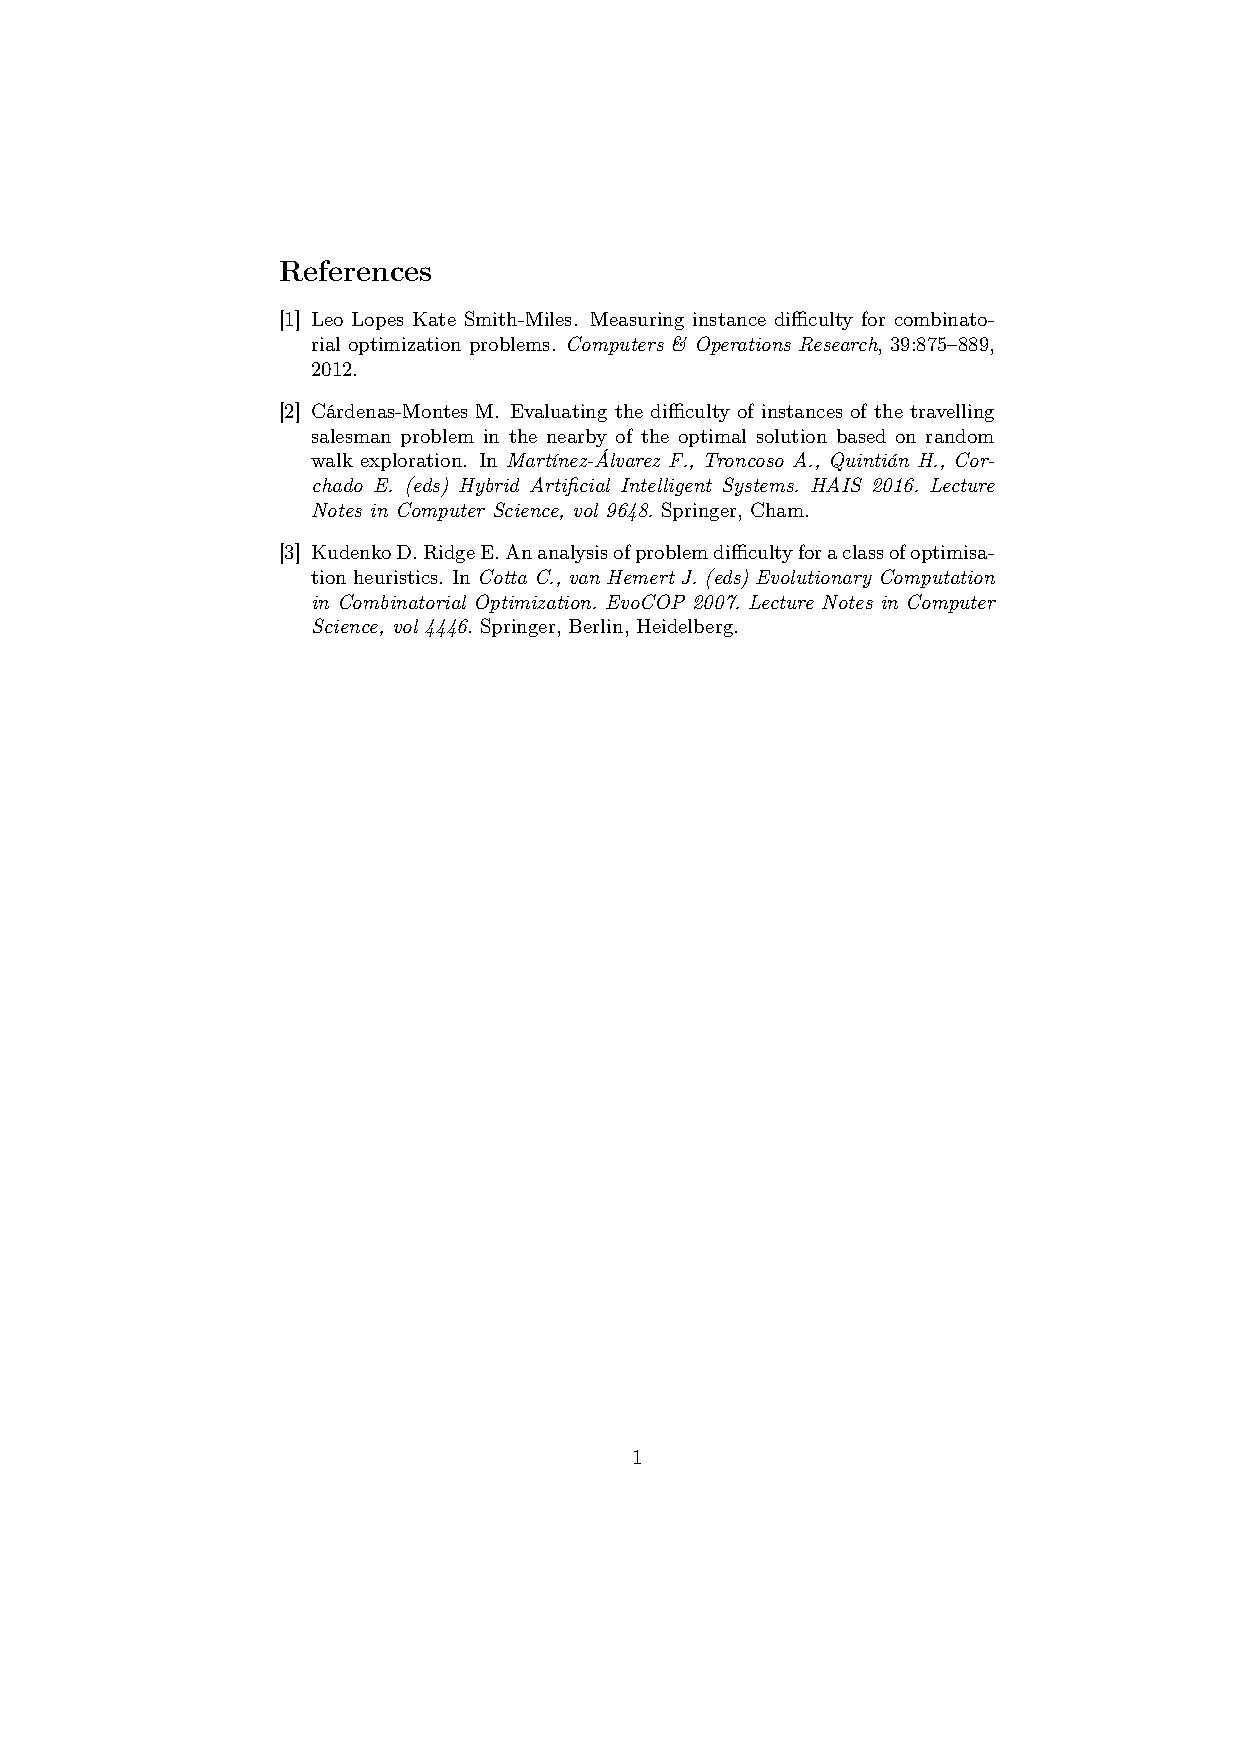
\includegraphics[width=\linewidth]{main}
        \caption{Menu principal}
    \end{subfigure}
    ~
    \begin{subfigure}{0.34\textwidth}
        \centering
        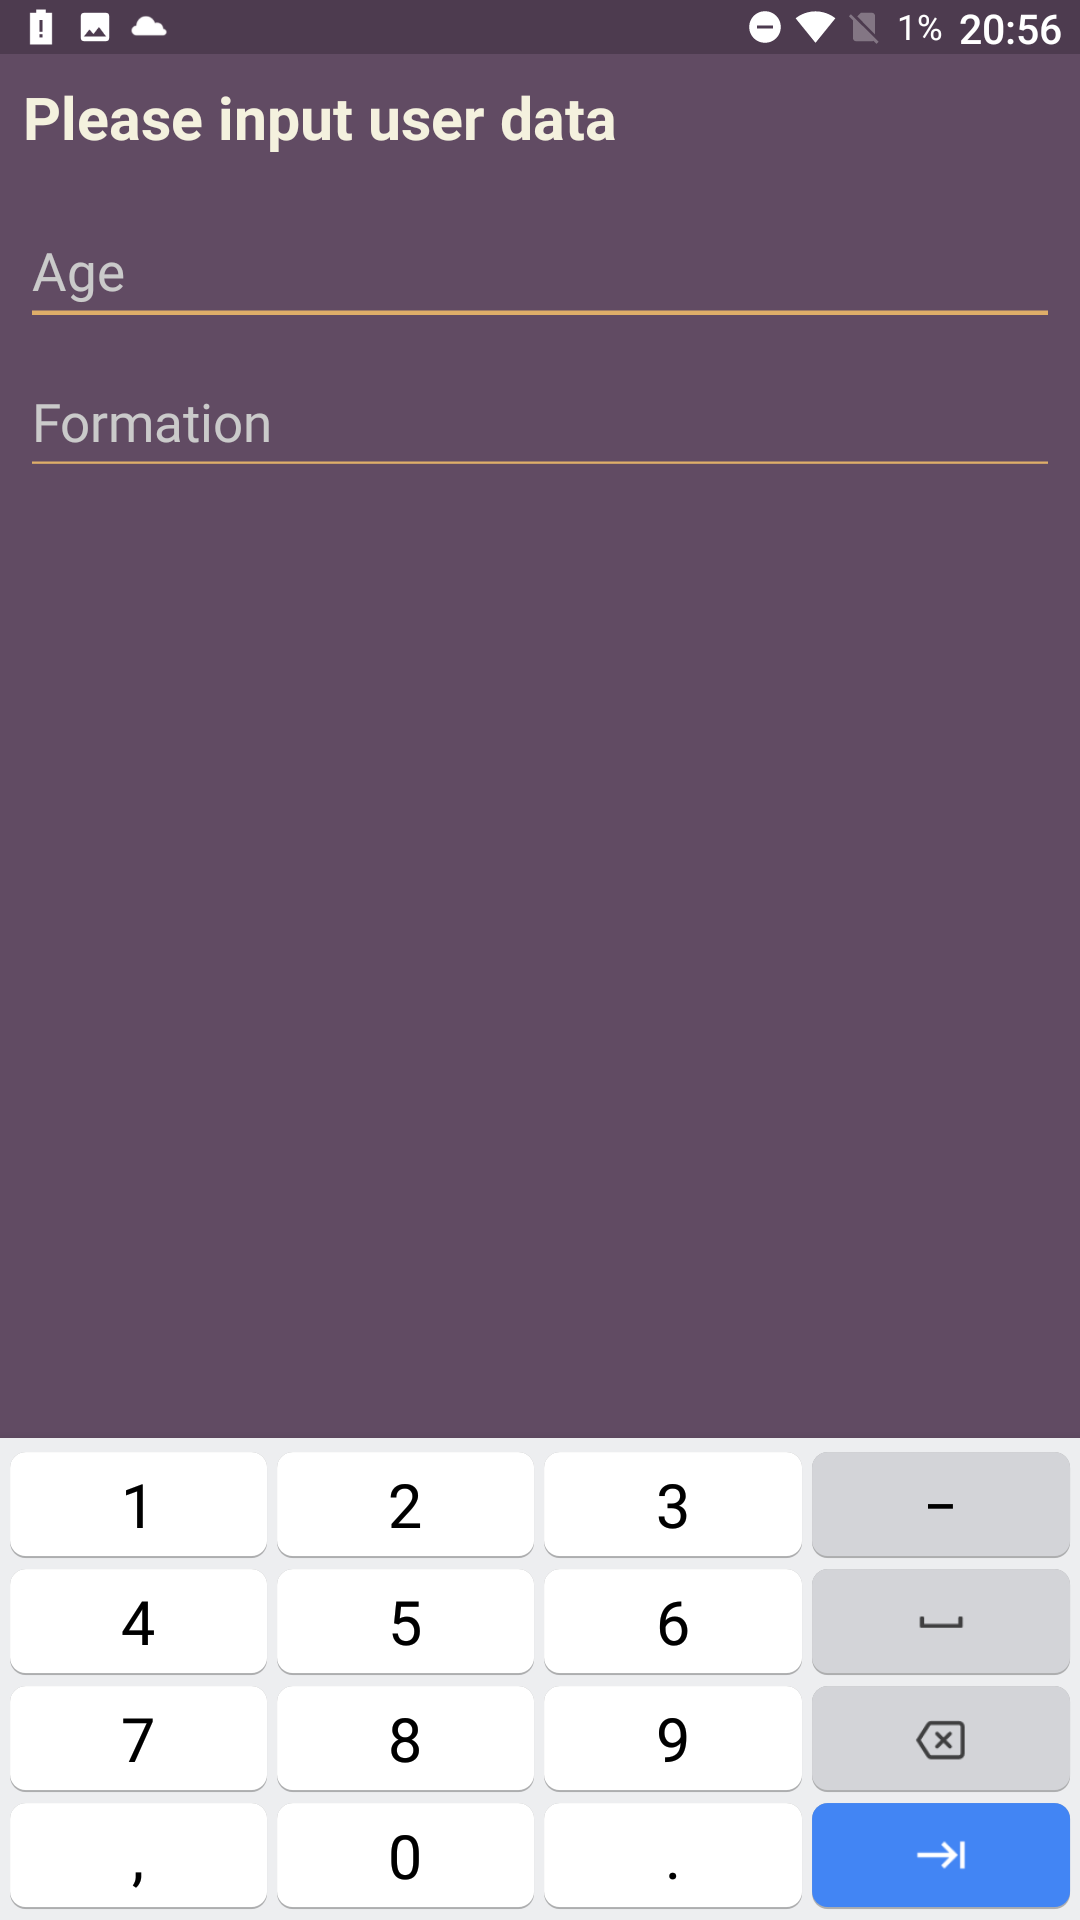
\includegraphics[width=\linewidth]{infor}
        \caption{Profil}
    \end{subfigure}
    ~
    \begin{subfigure}{0.34\textwidth}
        \centering
        
\includegraphics[width=\linewidth]{abou}
        \caption{About}
    \end{subfigure}
    ~
    \begin{subfigure}{0.34\textwidth}
        \centering
        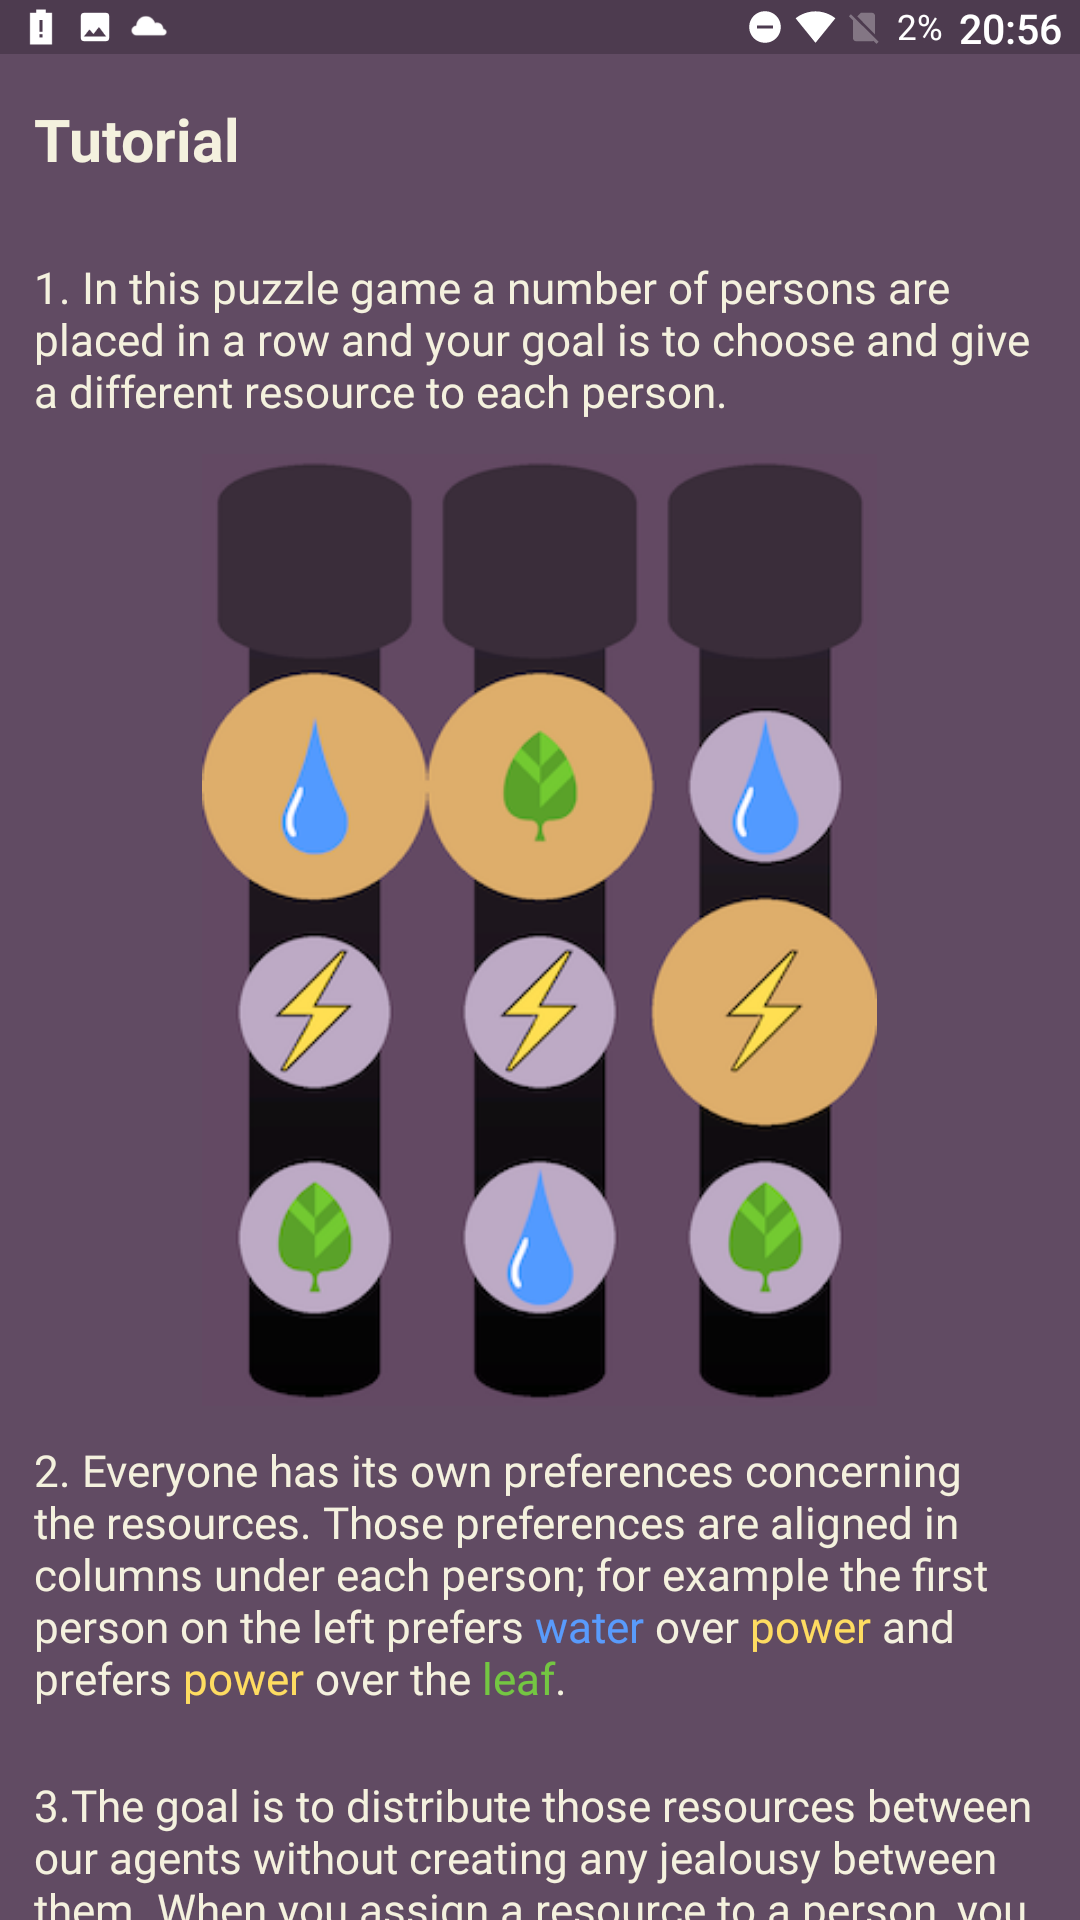
\includegraphics[width=\linewidth]{tuto}
        \caption{Tutoriel}
    \end{subfigure}
    \caption{Design final des menus de l'application}
    \label{fig-screen1}
\end{figure}
 
	\subsection{Le modèle du jeu}

\paragraph{}
Le package \texttt{models} contient les classes nécessaires à la représentation du jeu dans l'application. On y trouve la classe \texttt{Model}, appelée dès lors qu'il est demandé de faire une modification du modèle (assignation d'un objet à un des agents par exemple) ou encore de récupérer des informations du jeu comme le nombre d'agents d'un niveau. Cette classe stocke en effet la grille qui représente un niveau, comprenant les agents et les préférences. Le package contient également la définition de l'interface \texttt{IPiece}, implémentée par les classes \texttt{Preference} et \texttt{Actor} qui représentent respectivement les préférences et les agents.

 \begin{itemize}
\item définition d'une Pièce (Interface \texttt{IPiece}) : L’interface IPiece est composé de deux méthodes, la méthode getId qui retourne l'identifiant de la pièce et la méthode getPosition qui permet de retourner la position de la pièce sous forme d’un objet position qui contient les indices de la ligne et de la colonne dans lesquelles se trouve la pièce.   
\item définition d’un Acteur (Classe \texttt{Actor}) : La classe Actor implémente l'interface IPiece et toute ses méthodes, elle représente les agents du jeu.                                                                                                                                                                                                                                                                                                                                      
\item définition d’une Préférence (Classe \texttt{Préférence}) : La classe Préférence implémente également l’interface IPiece, on y ajoute cependant là deux entier, value : qui permet de déterminer de quel type est cette préférence et selectedby : qui permet de savoir si cette préférence est sélectionnée par un des agents et par quel agent elle l’est. 
\end{itemize}
\hfill \break
\begin{lstlisting}
private boolean isJealous(Preference[] P1,Preference[] P2){
    if (P1[0] == null){
        return false;
    }
    Preference P2pref = null;
    Preference P1pref = null;
    for (Preference pref:P1){
        if(pref.getSelectedby() != -1){
            P1pref = pref;
        }
    }
    for(Preference pref:P2){
        if(pref.getSelectedby() != -1){
            P2pref = pref;
        }
    }
    if(P1pref == null || P2pref == null){
        return false;
    }
    for(Preference pref:P2){
        if(pref.getValue() == P1pref.getValue()){
            if(pref.getPos().getCol() < P2pref.getPos().getCol()){
                return true;
            }
        }
    }
    return false;
}
\end{lstlisting}
Fonction de détection de la jalousie 

	\subsection{Design interface}
	
\paragraph{}
L’interface centrale de  l’application, l’aire de jeu de equity est un des composants principaux du projet et a donc suivit un certain nombre d'itérations qui seront décrites dans la partie suivante. Le premier objectif de cette interface était de pouvoir représenter le jeu sur un écran de smartphone en mode portrait.
\paragraph{}
Il a été déterminé très tôt dans le projet qu’une visualisation sous forme de grille serait nécessaire, chaque case de la grille représentant une préférence d’un des agents. Il a ensuite été décidé que les agents, représentés par des carrés, serait placé sur la gauche de la grille et leur préférences, représenté par des cercles, sur la même ligne que l’agent avec son objet préféré sur la gauche le plus proche de lui.
\paragraph{}
Il a ensuite été décidé que pour afficher la sélection d’une préférences par un des agents, un cercle de la couleur de l’agent serait dessiné derrière le cercle représentant la préférence en question, l'utilisateur peut donc choisir de sélectionner une certaine préférence en touchant l'icône correspondante. On note que le processus de sélection des ressources empêche de sélectionner plusieurs ressources pour un seul agent. A ce stade l’application est fonctionnelle.
\paragraph{}
La dernière modification structurelle de l’IHM consiste à optimiser l’espace qui est alloué à l’affichage des préférences des agents : L'affichage de la grille de jeu a été pivoté pour que les agents se trouvent en haut de l'écran, l'alignement des préférences se faisait donc de haut en bas, ce changement a donc permis d'utiliser une plus grande partie de la hauteur de l'écran du smartphone. En effet cette rotation de la grille a permis d'économiser une colonne en ajoutant une ligne ce qui est plus adapté à l’affichage en mode portrait.
\paragraph{}
les modifications suivantes de l’activité ont été soit esthétiques soit relevant de l’ajout de feature : tout d’abord l’interface a suivis un redesign complet, une harmonisation des couleurs et des formes pour la représentation de la plupart des éléments à dessiner. L’ajout de barres verticales pour chacun des agents, ce qui facilite la lisibilité et l’ajout de l’identifiant du niveau.
\paragraph{}
    Après avoir testé cette interface nous avons décidé que pour améliorer l'expérience de jeu nous devions rendre la détection d’affectation erroné plus aisée. Nous avons donc implémenté les solutions suivantes :
 l’affichage d’une couleur différente sur les ressources sélectionnés par deux agents ce qui permet au joueur de remarquer immédiatement si une assignation des ressources est impossible
La possibilité d’afficher en rouge les colonnes des agents jaloux, notons que cette fonctionnalité facilite grandement le jeu, elle est donc désactivé par défaut et le joueur a la possibilité d’appuyer sur un bouton pour activer cet affichage.
\paragraph{}
    Ces deux fonctionnalités facilitent grandement le gameplay mais nous pensons que ce compromis permet une expérience de jeu plus fluide et agréable pour l’utilisateur, un point qui nous semble essentiel pour la distribution de l’application. 


	\subsection{Interface GameView}
	
L'interface centrale de  l'application, l'ère de jeu de equity est un des composants principaux du projet, le canevas utilisé pour dessiner les agents et leur préférence s'organise de la façon suivante : les agents sont placé en haut de la surface sur une ligne horizontale, et leurs préférences sont arrangés verticalement, leur objet préféré étant le premier en partant du haut, derrière chaque agent est dessiné une bande verticale sur laquelle sont aligné les préférences 
\begin{figure}[h!]
    \centering
    \begin{subfigure}{0.23\textwidth}
        \centering
        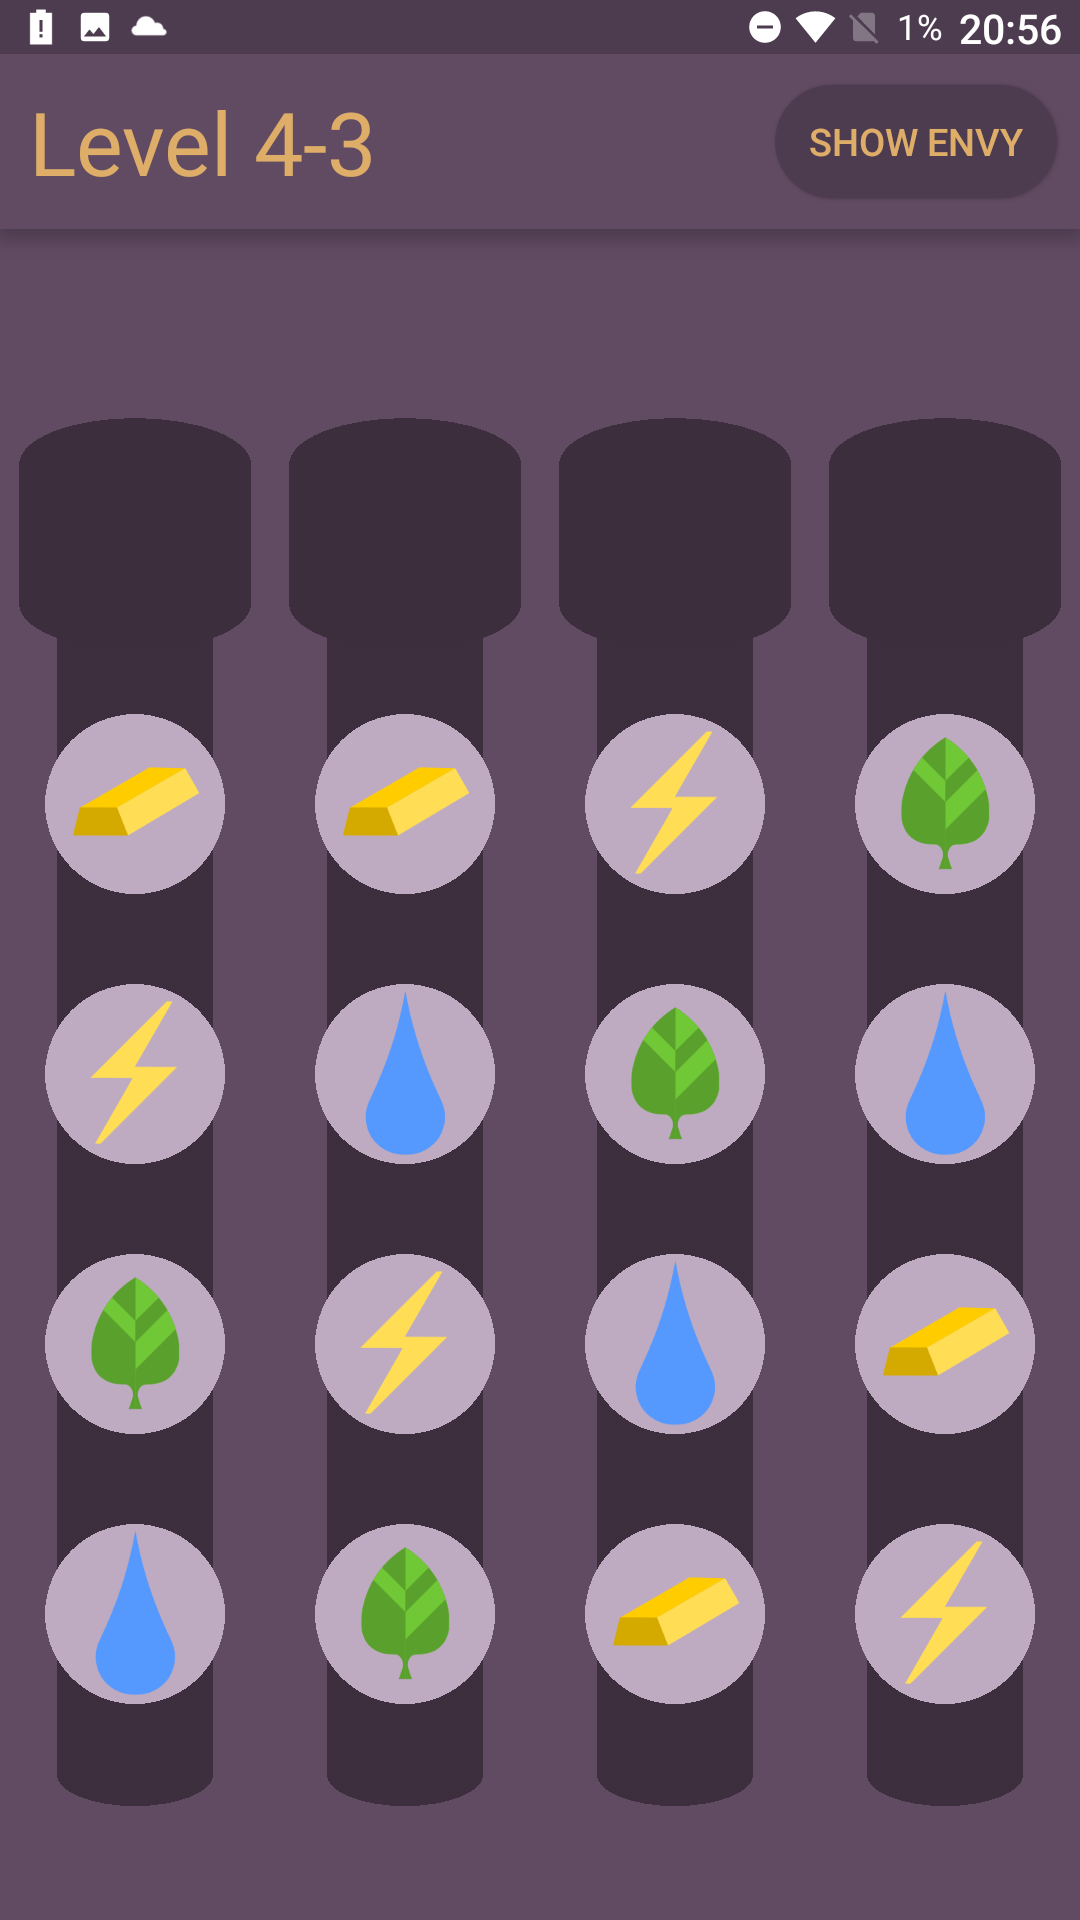
\includegraphics[height=2.5in]{g1}
        \caption{sélection}
    \end{subfigure}
        \begin{subfigure}{0.23\textwidth}
        \centering
        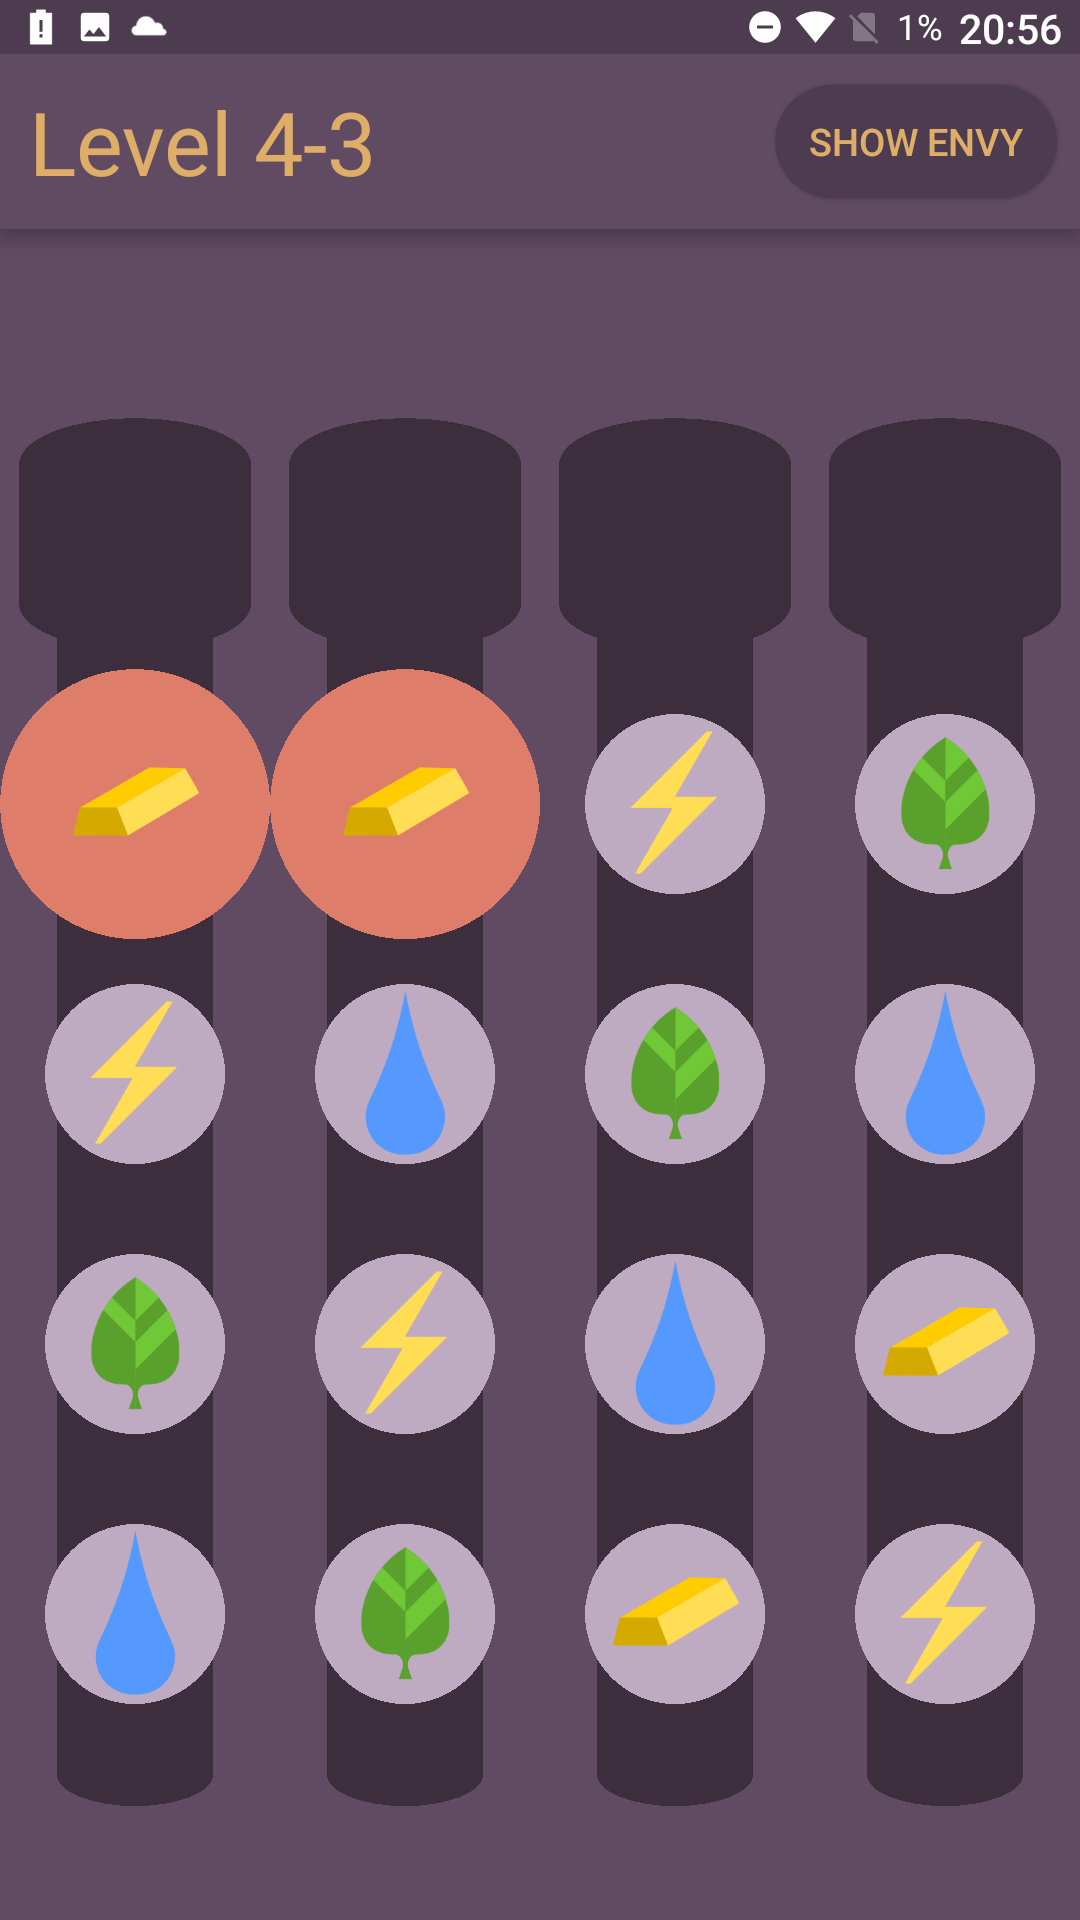
\includegraphics[height=2.5in]{g2}
        \caption{sélection}
    \end{subfigure}%
        \begin{subfigure}{0.23\textwidth}
        \centering
        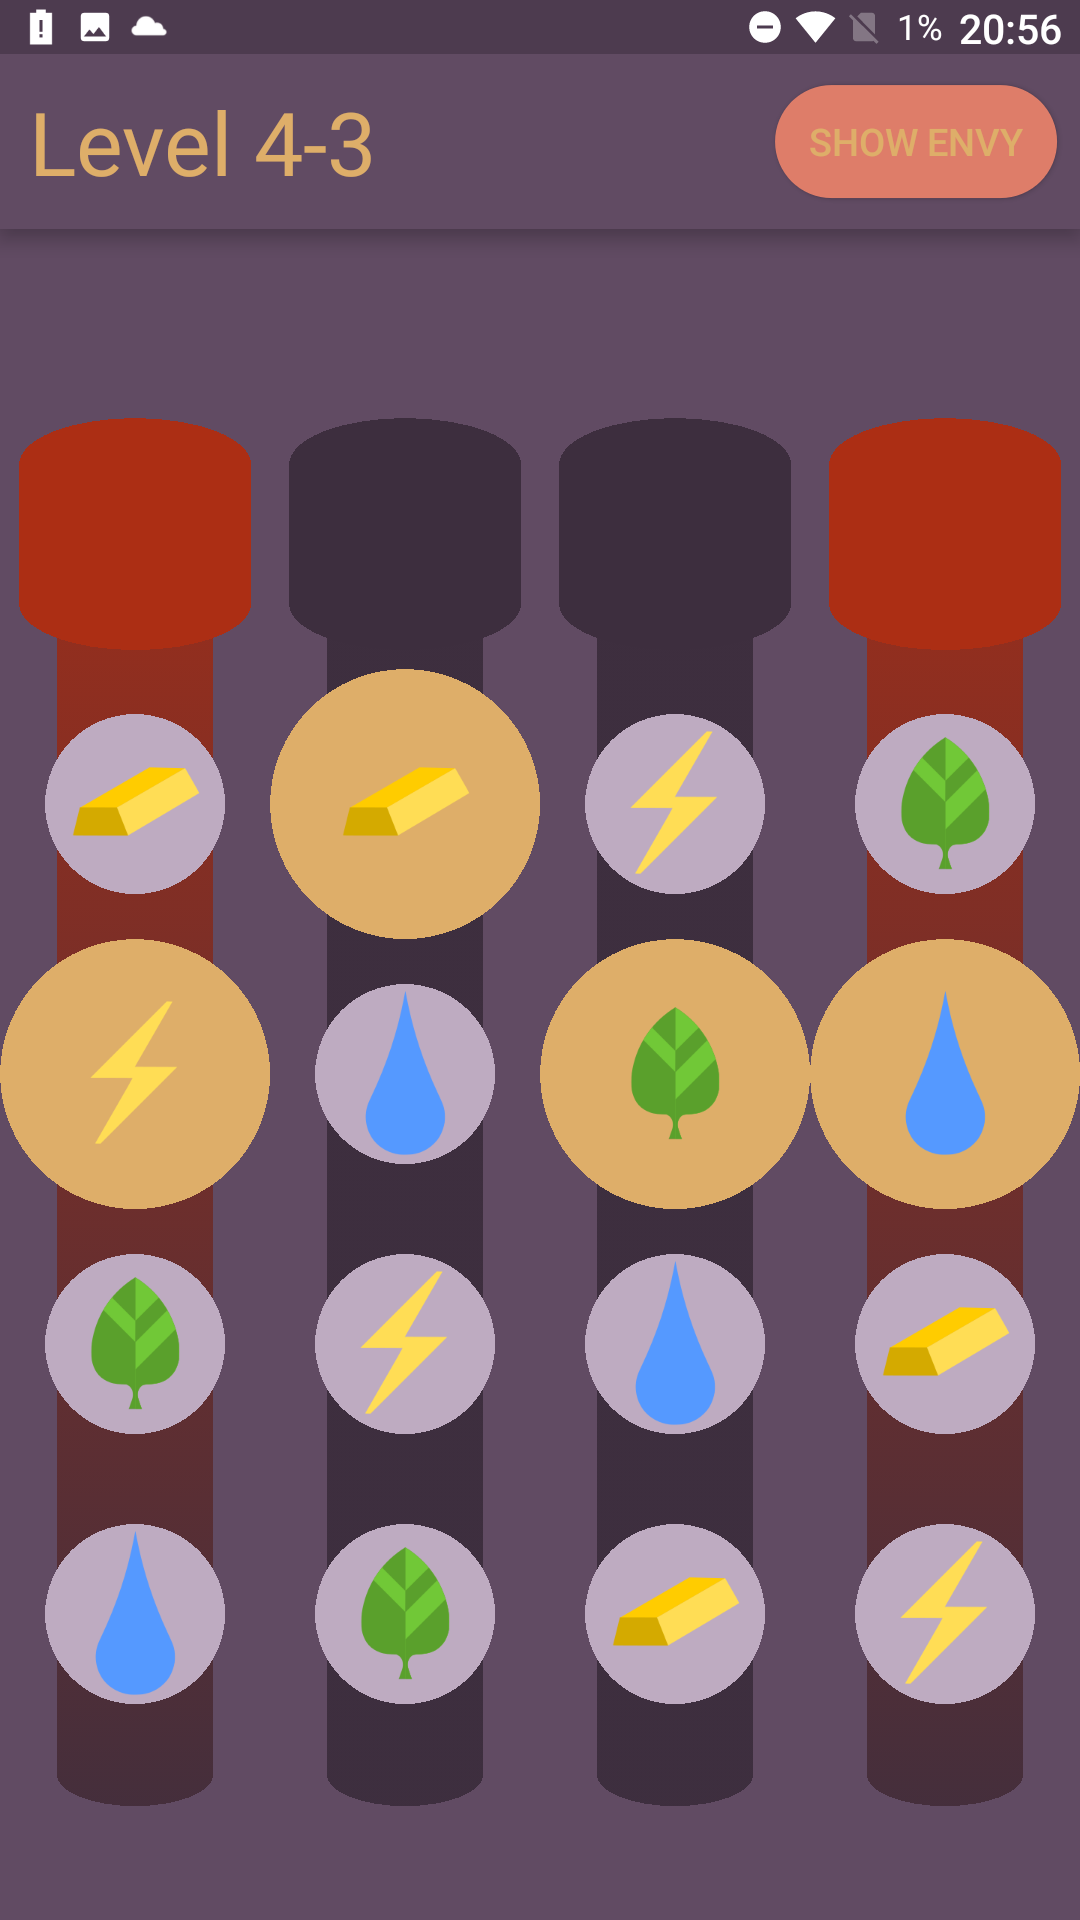
\includegraphics[height=2.5in]{g3}
        \caption{affichage}
    \end{subfigure}%
    \begin{subfigure}{0.23\textwidth}
        \centering
        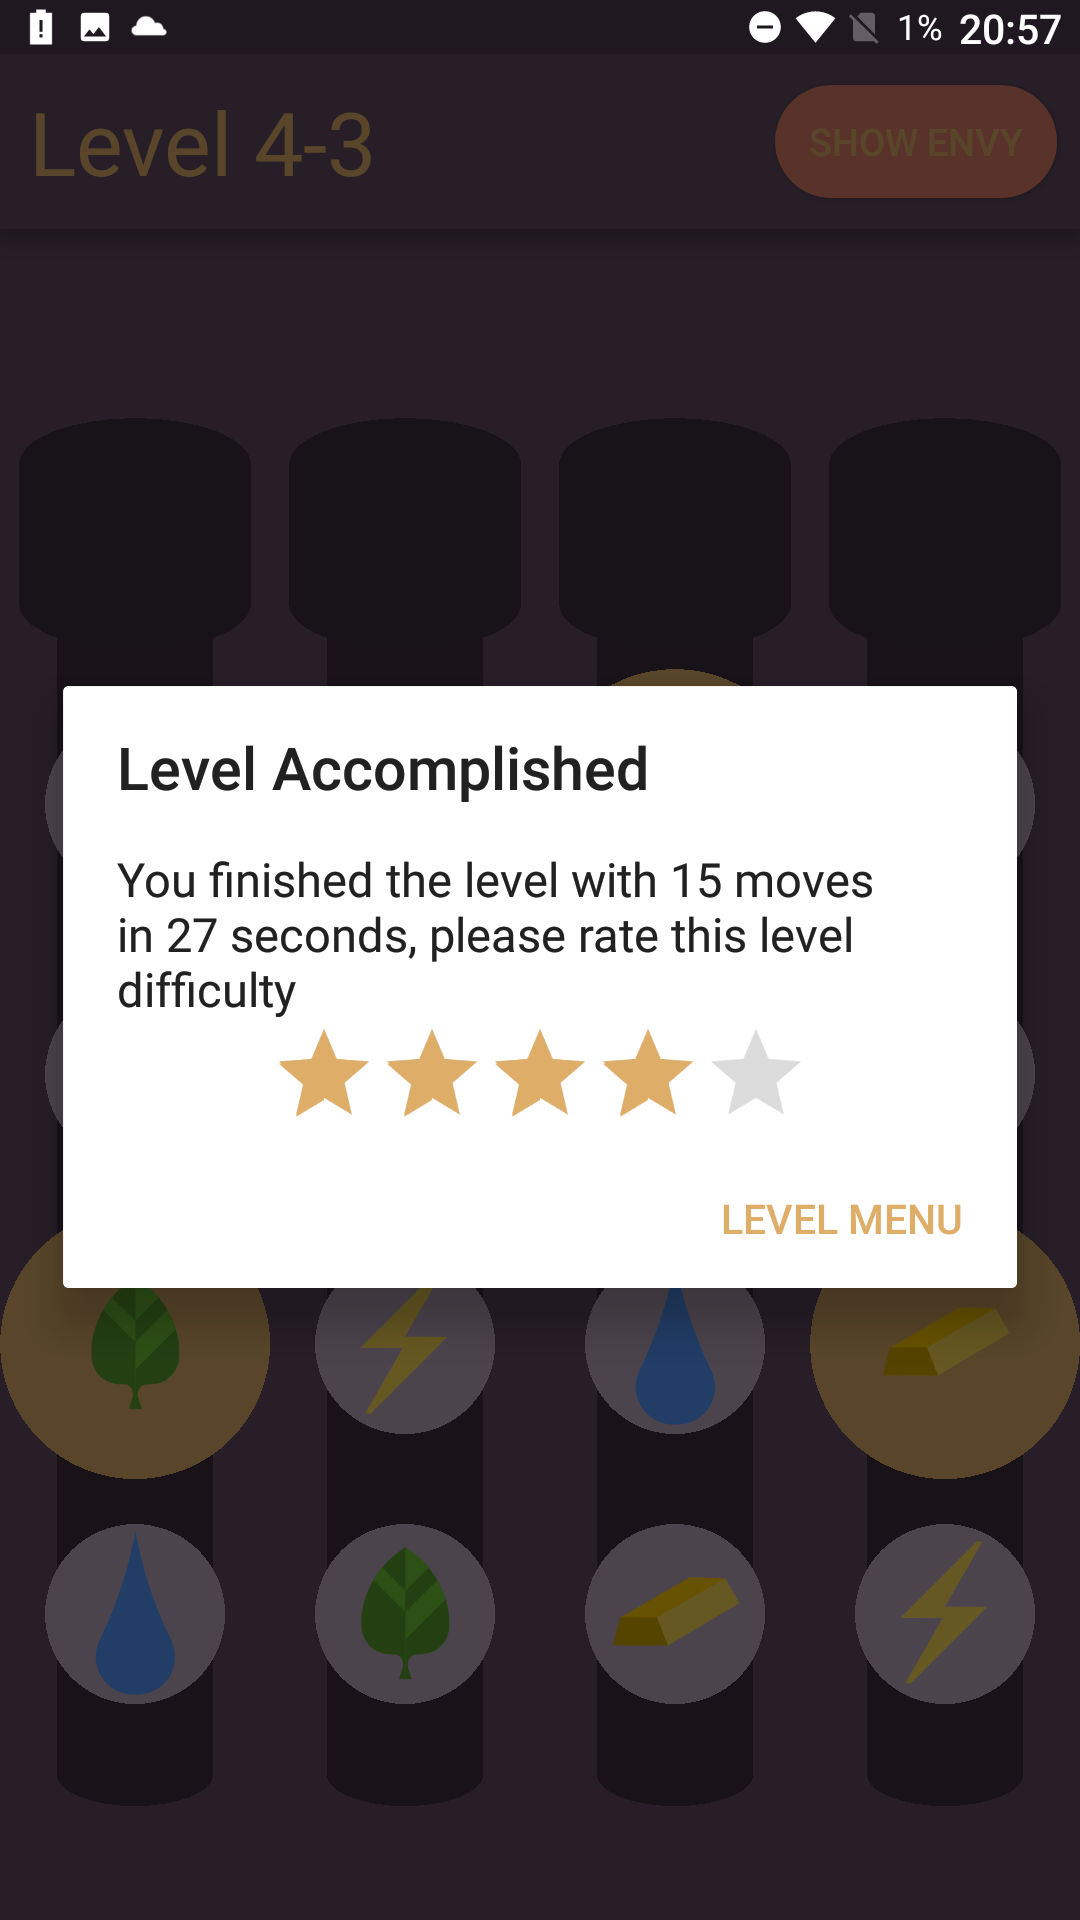
\includegraphics[height=2.5in]{g4}
        \caption{victoire}
    \end{subfigure}
    \caption{Exemple Gameview}
\end{figure}

	\subsection{Récupération des données}
	
	\paragraph{}
	L’analyse de diverses instances du problème nous a permis donc de dégager plusieurs métriques, qui peuvent être utilisées pour essayer de prédire la difficulté de nos niveaux. Cependant, il nous fallait confronter ces prédictions avec des données réelles , qui seraient justement basé sur ces critères, et ce afin de trouver si oui ou non, il existait une corrélation entre la difficulté d’un niveau et ces derniers. 
	\paragraph{}
Une fois l’application mobile réalisée, nous avions donc décidé de la faire tester sur un public de taille variante et diverse, pour recueillir assez de données. Mais nous avions besoin d’un moyen de les écrire quelque part , la contrainte étant que l’utilisateur allait jouer sur son téléphone. Il nous fallait donc envoyer ces informations sur une sorte de base de données. Notre regard s’est alors porté sur l’API Google Sheets qui nous offrait une relaxation de cette contrainte.

\paragraph{Googlesheets}
Nous avons donc intégré dans l’application mobile, une solution permettant l’envois de diverses données joueurs qui étaient enregistrées lors de la résolution d’une instance. l’API Google Sheets permet l’écriture/lecture de données sur une Google Sheet via différentes plateformes : application mobile, site web, programme python, etc… 
En ce qui nous concerne, notre but est d’envoyer les différentes métriques abordées précédemment sur une Google Sheet avec diverses informations sur l’utilisateur pour ensuite les analyser et appliquer une régression dessus.

\paragraph{}
La communication entre la feuille et notre application est géré via l’API, et elle est sécurisé. En effet l’API utilise le protocole OAuth 2.0 pour autoriser les communications. Nous avons donc besoins d’identifiants , deux moyen sont disponibles :
 \begin{itemize}
\item l’usage d’une Clé API
\item l’usage d’un compte de service Google
\end{itemize}
Néanmoins, la première méthode requiert une confirmation de l’utilisateur à chaque fois qu’il envoie des données via son téléphone car l’application demandera la permission d'interagir avec la feuille sous le compte de l’utilisateur. Nous avons donc opté pour la seconde solution qui user d’un compte de service dédié à notre application. L’application interagira via ce compte sans demander la confirmation de l’utilisateur, ce qui est crucial pour l’envie de l’utilisateur à vouloir tester notre application sur une courte durée/longue durée.
Dans les deux cas, un fichier JSON est créé et il contiendra les informations nécessaire pour créer nos identifiants.

\paragraph{}
L’intégration de cette solution dans notre application se traduit donc par deux classes:
 \begin{itemize}
\item La classe SheetsServiceUtil
\item La classe GoogleSheetsWriteUtil
\end{itemize}
\paragraph{}
La première classe java SheetsServiceUtil contient une unique méthode getSheetsService qui permet la création d’une instance de l’objet Sheet qui est l'intermédiaire pour écrire et lire via l’API. Cette instance contiendra les identifiants nécessaire à l’autorisation de la communication entre l’application et la feuille.
\paragraph{}
La deuxième classe java GoogleSheetsWriteUtil contient toutes les méthodes qui seront appelées pour l’écritures de nos données. 
La méthode setup() permet entre autre la création d’une instance de l’objet Credential, à partir de notre fichier JSON qui est contenu dans les ressources de notre applications (pour rappel, on accède aux ressources de nos applications via ctx.getRessourses();). Cette instance est ensuite passée en paramètre dans la méthode getSheetsService de notre classe SheetsServiceUtil qui retournera un objet Sheets, sur lequel toute nos méthodes agiront par la suite.
Par ailleurs, nous récupérons aussi les données du profil utilisateur enregistré si elles existent pour permettre de détecter la modification d’un profil.
\paragraph{}
Nous utilisons des AsyncTask pour envoyer nos données. En effet il est impossible sous android de faire des opérations réseaux ( transfert de données ) , sous le thread principale, on utilise donc des AsyncTask pour le faire en background. Cela nous évite des lags au niveau de l’interface qui est entièrement gérée par le main thread.
et ça reste invisible à l’oeil de l’utilisateur ce qui est à nouveau crucial quant au côté agréable et fluide de son expérience.
\paragraph{}
Nous avons donc trois static private Class dans SheetsServiceUtil qui héritent tous de la class AsyncTask , une classe d’Android qui permet de lancer des threads aisément : 
 \begin{itemize}
\item WriteUserInfoAsyncTask
\item ModifyUserInfoAsyncTask
\item WriteUserEvalAsyncTask
\end{itemize}
Ces trois classes implémentent ainsi la méthode protected doInBackground , qui prend en paramètre un string data, c’est à dire les données à envoyer, et qui permet leur exécution en tâche de fond.
Nous appelons donc à l'intérieure les méthodes de l’API de Google Sheets pour update (pour modifyUserInfoAsync) 
ou écrire de nouvelles données (pour WriteUserEvalAsyncTask et ModifyUserInfoAsyncTask) dans notre feuille en utilisant l’instance de la classe Sheets que l’on avait créé au préalable.
\hfill \break 
\begin{lstlisting}[tabsize=3]
private static class WriteUserInfoAsyncTask extends 
AsyncTask<String, Void, Void>{
	@Override
	protected Void doInBackground(String... data) {
		ValueRange body = new ValueRange()
                    .setValues(Arrays.<List<Object>>asList(
                            new List[]{Arrays.asList(data)}
                    ));
		try {
			AppendValuesResponse result = sheetsService.spreadsheets()
			.values().append(SPREADSHEET_ID, "User_Info_2!A1", body)
			.setValueInputOption("USER_ENTERED")
			.execute();
			Object userPos = result.getUpdates().get("updatedRange");
			prefs.edit().putString("userPos", (String) userPos).apply();
		} catch (IOException e) {
			Log.w("GoogleSheet", "Error during user info write; 
			rescheduling");
			failedUserInfo = data;
			e.printStackTrace();
		 }
		return null;
	}
}
\end{lstlisting}
Fonction WriteUserInfoAsyncTask
\paragraph{}
Comme il est possible que l’écriture des données sur la feuille puisse échouer (problème de réseau, téléphone non connecté à internet, etc...) , il est nécessaire de sauvegarder les données non envoyées pour permettre une planification d’un renvois plus tard. Il existe donc deux variables dans notre classe SheetsServiceUtil pour cela : 
failedEvaluation si l’écriture d’une évaluation échoue
failedUserInfo si l’écriture/modification du profil utilisateur échoue
\paragraph{}
Avant toute nouvelles écritures, il faut donc vérifier s’il n’en existe pas qui ont échouées.
Pour cette raison, nous avons créé trois méthodes : WriteUserInfo(String data), ModifyUserInfo(String data) , WriterUserEval(String data), qui appelle toujours au début une méthode “CheckFailures” qui verifie si failedEvaluation et failedUserInfo sont vide ou non. Si elles ne le sont pas, alors on crée de nouvelles asyncTask pour renvoyer ces données. Et dans tous les cas, on crée de nouvelles AsyncTask correspondant à la méthode qui est appelé (par exemple WriteUserInfoAsyncTask pour la méthode WriteUserInfo) pour les nouvelles données passées en paramètre de ces méthodes.
\hfill \break
\begin{lstlisting}[tabsize=3]
public void writeUserEvaluation(String... data) {
	this.checkFailures();
	new WriteUserEvaluationAsyncTask().execute(data);
}
\end{lstlisting}
Méthode WriteUserEvaluation
	
\end{document}



